\documentclass[12pt,a4paper]{report}
\usepackage{geometry}
\geometry{
	a4paper,
	total={170mm,257mm},
	left=20mm,
	top=20mm,
}
\usepackage{graphicx}
\usepackage{pdfpages}

\usepackage{polski}
\usepackage[utf8]{inputenc}

\begin{document}
	
	\begin{titlepage}
		\newgeometry{top=5.5cm, bottom=3cm}
		
		\centering
		{\huge\bfseries Logika układów cyfrowych lab.\par}
		
		\vspace{0.5cm}
		Prowadzący: Antoni Sterna (E02-38m, wtorek 17:05) \\
	
		\vspace{1.1cm}
		{\Large sprawozdanie 1 - 2017.10.10\par}
		\vfill
		
		{\large\bfseries Jakub Dorda 235013\par}
		{\large\bfseries Marcin Kotas 235098\par}
		
		\vspace{1cm}
		\today \\ \LaTeX
		
		\restoregeometry
	\end{titlepage}
	
	%wprowadzenie
	
	
	%tabela prawdy
	
	
	%minimalizacja
	
	
	%wzory
	
	
	%schemat ideowy układu
	{\large\bfseries Schemat ideowy układu na bramkach NAND}
	\vspace{0.5cm}
	\begin{center}
		\makebox[\textwidth]{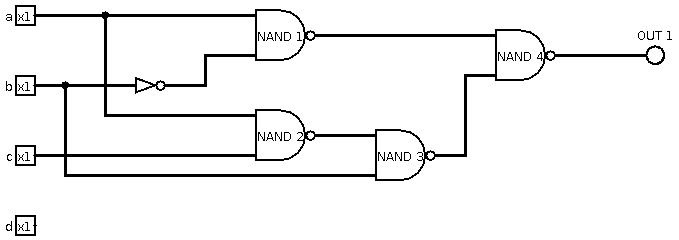
\includegraphics[width=\paperwidth - 40mm]{schem/circuit.png}}
	\end{center}
	
	{\large\bfseries Schemat ideowy układu na bramkach NOR}
	\vspace{0.5cm}
	\begin{center}
		\makebox[\textwidth]{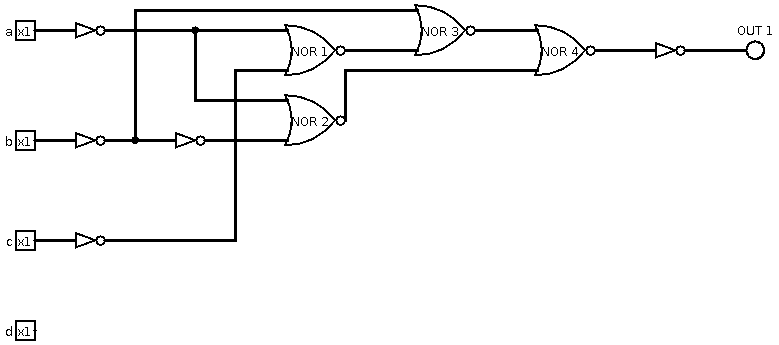
\includegraphics[width=\paperwidth - 40mm]{schem/circuit2.png}}
	\end{center}
	Wszystkie wejścia poprowadzone przez bramki NOR lub sygnał z wyjść 0 przełączników. 
	
	
	%wnioski
	
	
\end{document}